\section{Validierung}
In diesem Kapitel geht es darum, Anforderungen und Eigenschaften des Aktor- und Sensorbausteins zu testen.
\subsection{Sensorbaustein}
\subsubsection{ESD Test}
Der Sensorbaustein wird wie eine Unterputzsteckdose verbaut und die Frontplatte dient als User-Interface. 
Genauer bedeutet es, dass der Benutzer, die Touchflächen der Frontplatte berühren muss, um mit dem Sensorbaustein zu interagieren. 
Durch das berühren kann es jedoch zu elektrostatischen Entladungen kommen, die der Sensorbaustein überstehen muss.
Deswegen wurde mithilfe eines ESD-Tests, getestet bis zu welchem Prüfschärfegrad, also bis zur welcher Entladespannung der Sensorbaustein funktioniert.
In der Tabelle \ref{tab: ESD_Testablauf} sind die Prüfschärfegrade und deren Spannungen abgebildet.
Für den Test wurde die Kontaktentladung genommen, mit welcher eine Entladung über einen Finger nachgestellt wird.\\
Der Testablauf war wie folgt \cite{schleuniger_emv_w8_2020}:\\
\\
- Beginn beim tiefsten Schärfegrad\\
- 1 Entladung/s\\
- mind. 10 Entladungen, jeweils auf jeder Touchfläche\\


\begin{figure}[H]
	\centering
	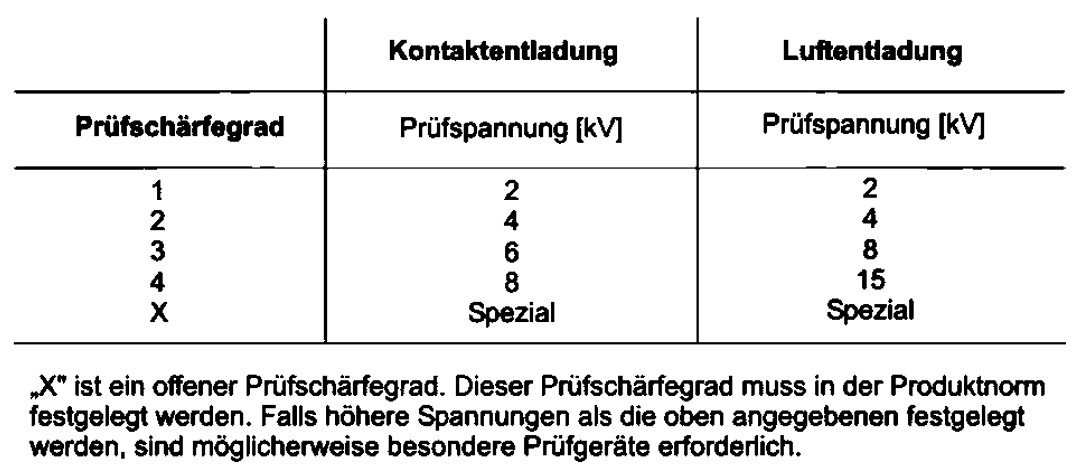
\includegraphics[width=0.8\textwidth]{graphics/ESD_Testablauf.jpg}
	\caption{ESD Testablauf \cite{schleuniger_emv_w8_2020}}
	\label{tab: ESD_Testablauf}
\end{figure}

Das Resultat war, dass der Sensorbaustein beim Prüfschärfegrad 4 Schaden nahm. Bei geringeren Spannungen war er funktionstüchtig. Was bedeutet, dass der Sensorbaustein Prüfschärfegrad 3 mit 6\,kV erreicht hat. Der Schaden beim Grad 4 war sichtbar und befand sich beim Seriell/UART-Wandler (Abbildung: \ref{pic: ESD_Schaden}), was nicht zu erwarten war. Der betroffene Pin war die Spannungsversorgung des IC's, dazu wurden direkt die 5\,V der Eingangsspeisung genommen, die Entweder über USB oder Pins angeschlossen wird. Beide Spannungsversorgungen sind miteinander verbunden, da in der Anwendung nur eines von beidem verwendet wird. Theoretisch wäre es auch möglich gewesen die 3.3\,V als Versorgung des Seriell/UART-Wandlers zu nehmen, die Frage ist, ob dann der gleiche Schaden aufgetreten wäre. Die Schutzdioden welche Über- und Unterspannung ableiten sind mit Ground bzw. 3.3\,V verbunden und nur der Seriell/UART-Wandler und der DC/DC Wandler sind an der 5\,V Speisung angeschlossen. Schlussendlich ist der Strom über den Seriell/UART-Wandler abgeflossen und hat ihn zerstört.

\begin{figure}[H]
	\centering
	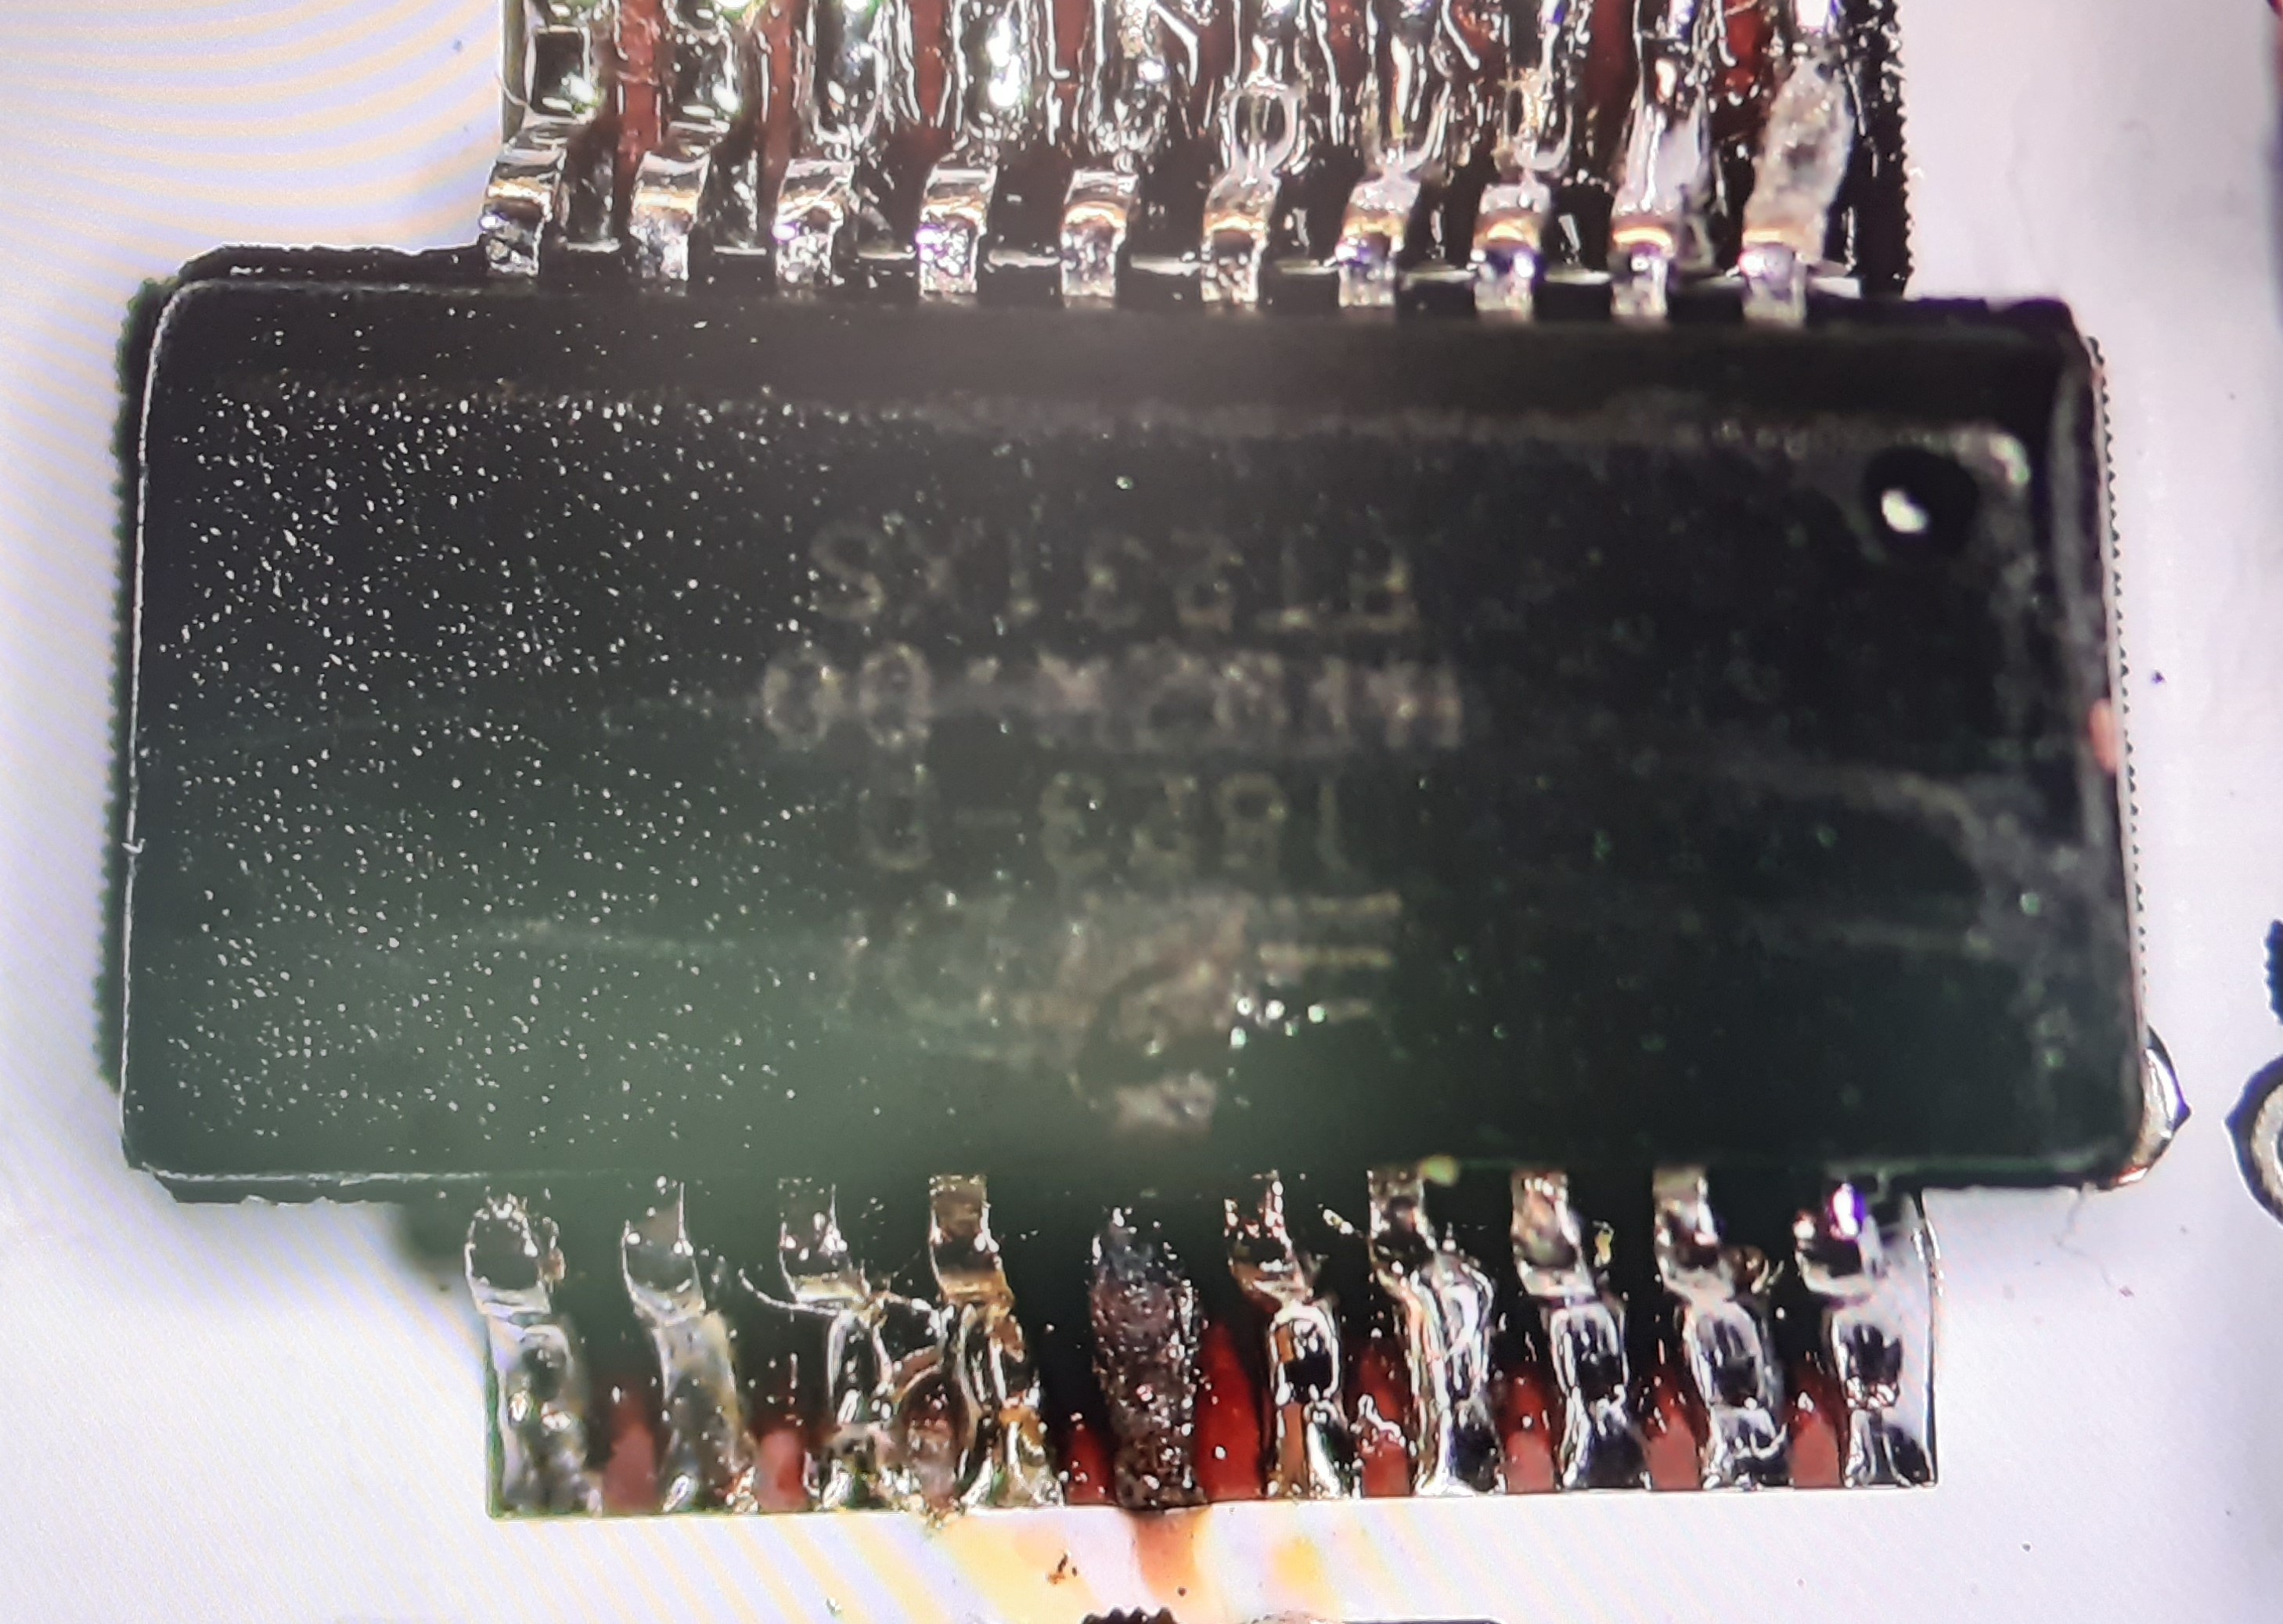
\includegraphics[width=0.8\textwidth]{graphics/ESD_Schaden.jpg}
	\caption{Der Schaden am Seriell/Uart-Wandler welcher, wegen des ESD Tests mit Prüfschärfegrad 4 zu Stande kam}
	\label{pic: ESD_Schaden}
\end{figure}

\subsubsection{Energieverbrauch des Sensorbausteins} \label{energie_sensorbaustein}
Der Sensorbaustein wurde unter folgenden Bedingungen gemessen:
\begin{enumerate}
	\item Ungeschalteter Normalzustand (Abbildung: \ref{pic: Sensorbaustein_ungeschaltet}) \\(Der Sensorbaustein wird nicht bedient und hat eine Verbindung mit einem WLAN Netzwerk) \\
	Der Sensorbaustein hat eine mittlere Leistungsaufnahme von ca. 370\,mW. Auffällig ist, dass die Leistung mit einer Periode von 10\,s schwankt, was dem zu Programm zugrunde liegt, denn die Temperaturmessung, denn das Status LED toggelt alle 10\,s, um anzuzeigen, dass die Temperatur nach 10\,s wieder gemessen wird. Unregelmäßige Leistungssprünge von bis zu ca. 400\,mW kommen häufiger vor, was wahrscheinlich durch das WLAN ausgelöst wird.
	\\
	\item Geschalteter Normalzustand (Abbildung: \ref{pic: Sensorbaustein_geschaltet})\\ (Der Sensorbaustein wird bedient und hat eine Verbindung mit einem WLAN Netzwerk)\\
	In den Zeiten um ca. 35\,s, 60\,s und 85\,s werden alle Vier Taster betätigt, die Leistungsaufnahme steigt um 10\,mW von vorher 370\,mW auf ca. 380\,mW, was vertretbar ist.
	\\
	\item Keine Verbindung (Abbildung: \ref{pic: Sensorbaustein_keine_Verbindung})\\ (Der Sensorbaustein findet kein zulässiges WLAN Netzwerk)\\
	In diesem Zustand hat der Sensorbaustein eine mittlere Leistungsaufnahme von 930\,mW, was beträchtlich ist. Dies ist daran geschuldet, dass der Sensorbaustein vermutlich seine seine Signalstärke erhöht, um ein Netzwerk zu finden. Deswegen wird nicht empfohlen, den Sensorbaustein, in diesem Zustand zu lassen.
\end{enumerate}


\begin{figure}[H]
	\centering
	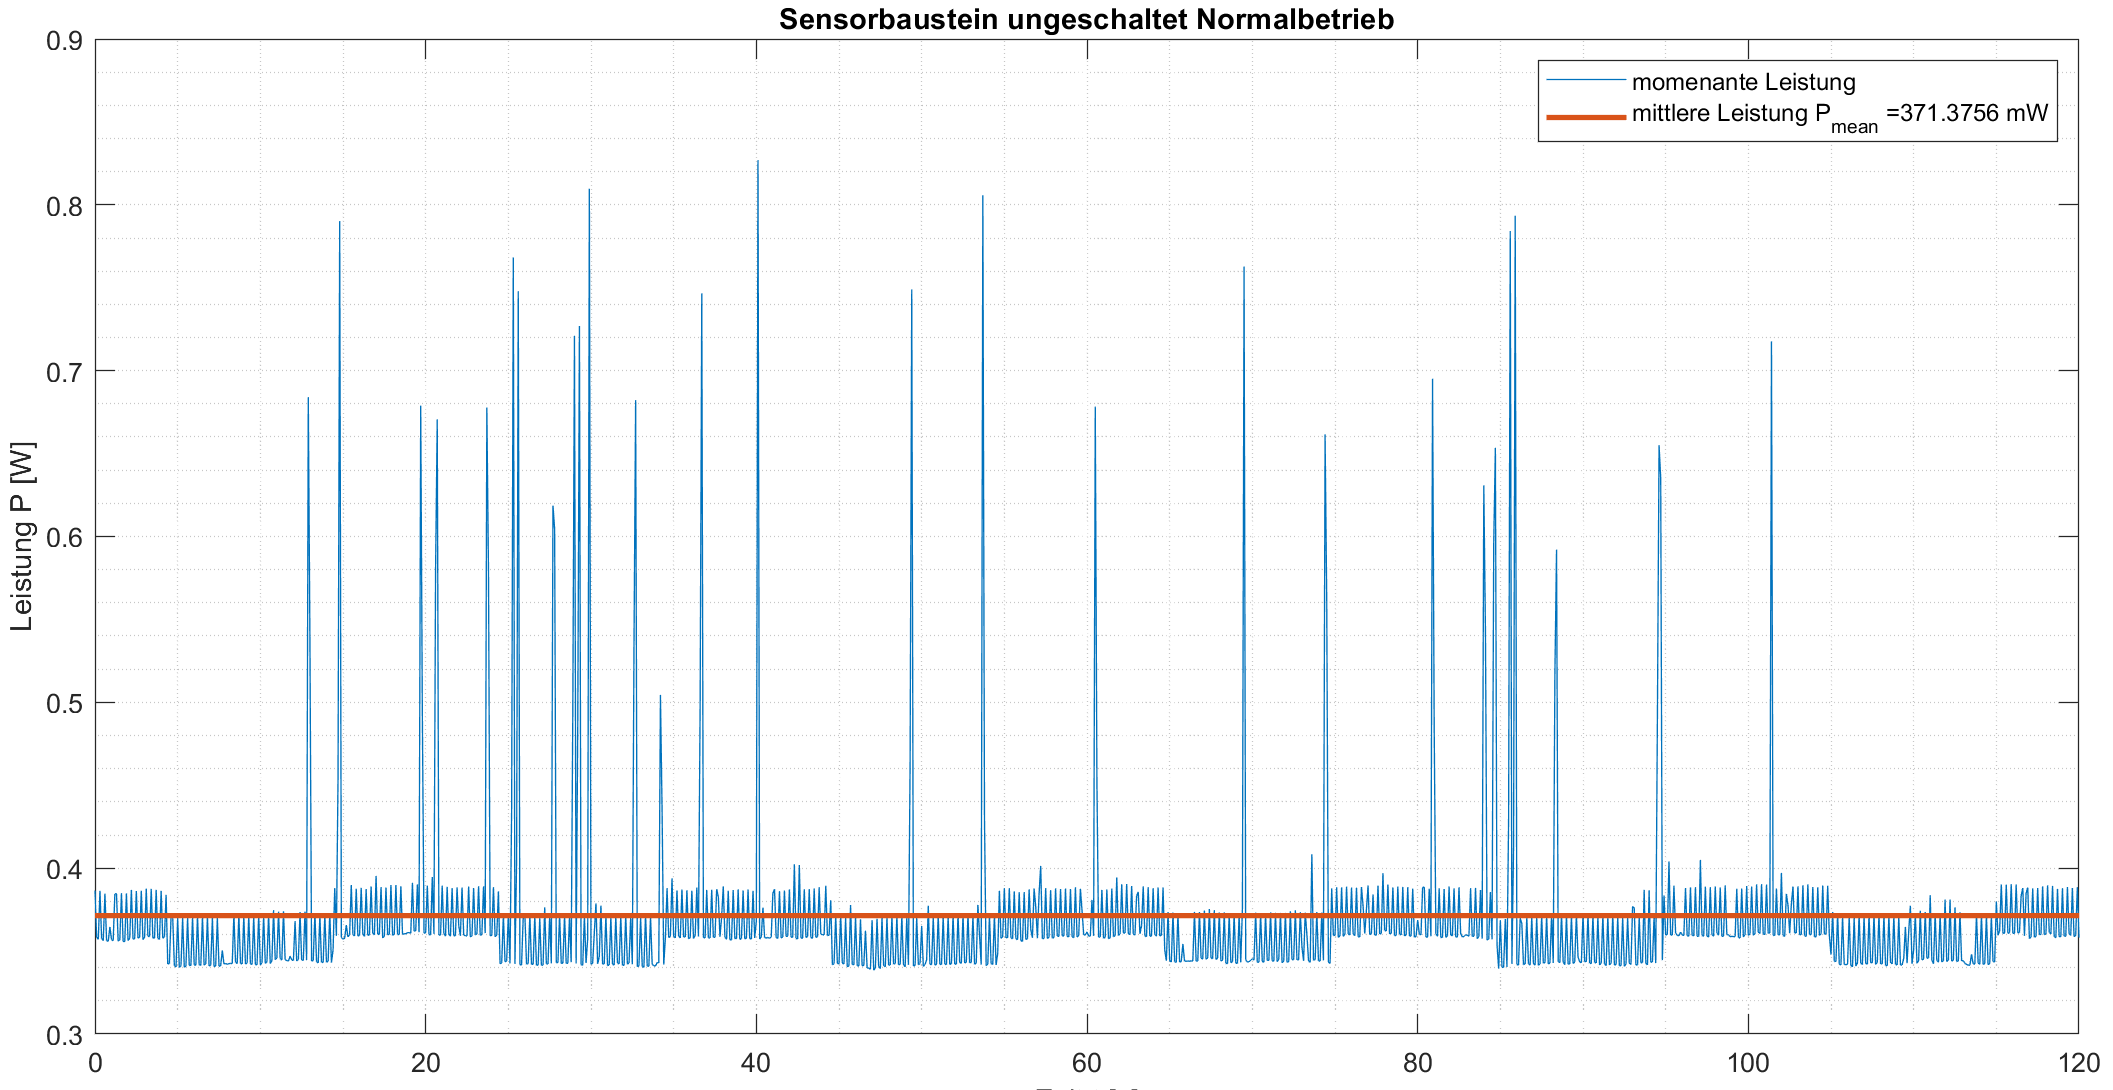
\includegraphics[width=1\textwidth]{graphics/Sensorbaustein_ungeschaltet.png}
	\caption{Die Leistung des Sensorbausteins, wenn er nicht bedient wird und mit dem Netzwerk verbunden ist}
	\label{pic: Sensorbaustein_ungeschaltet}
\end{figure}

\begin{figure}[H]
	\centering
	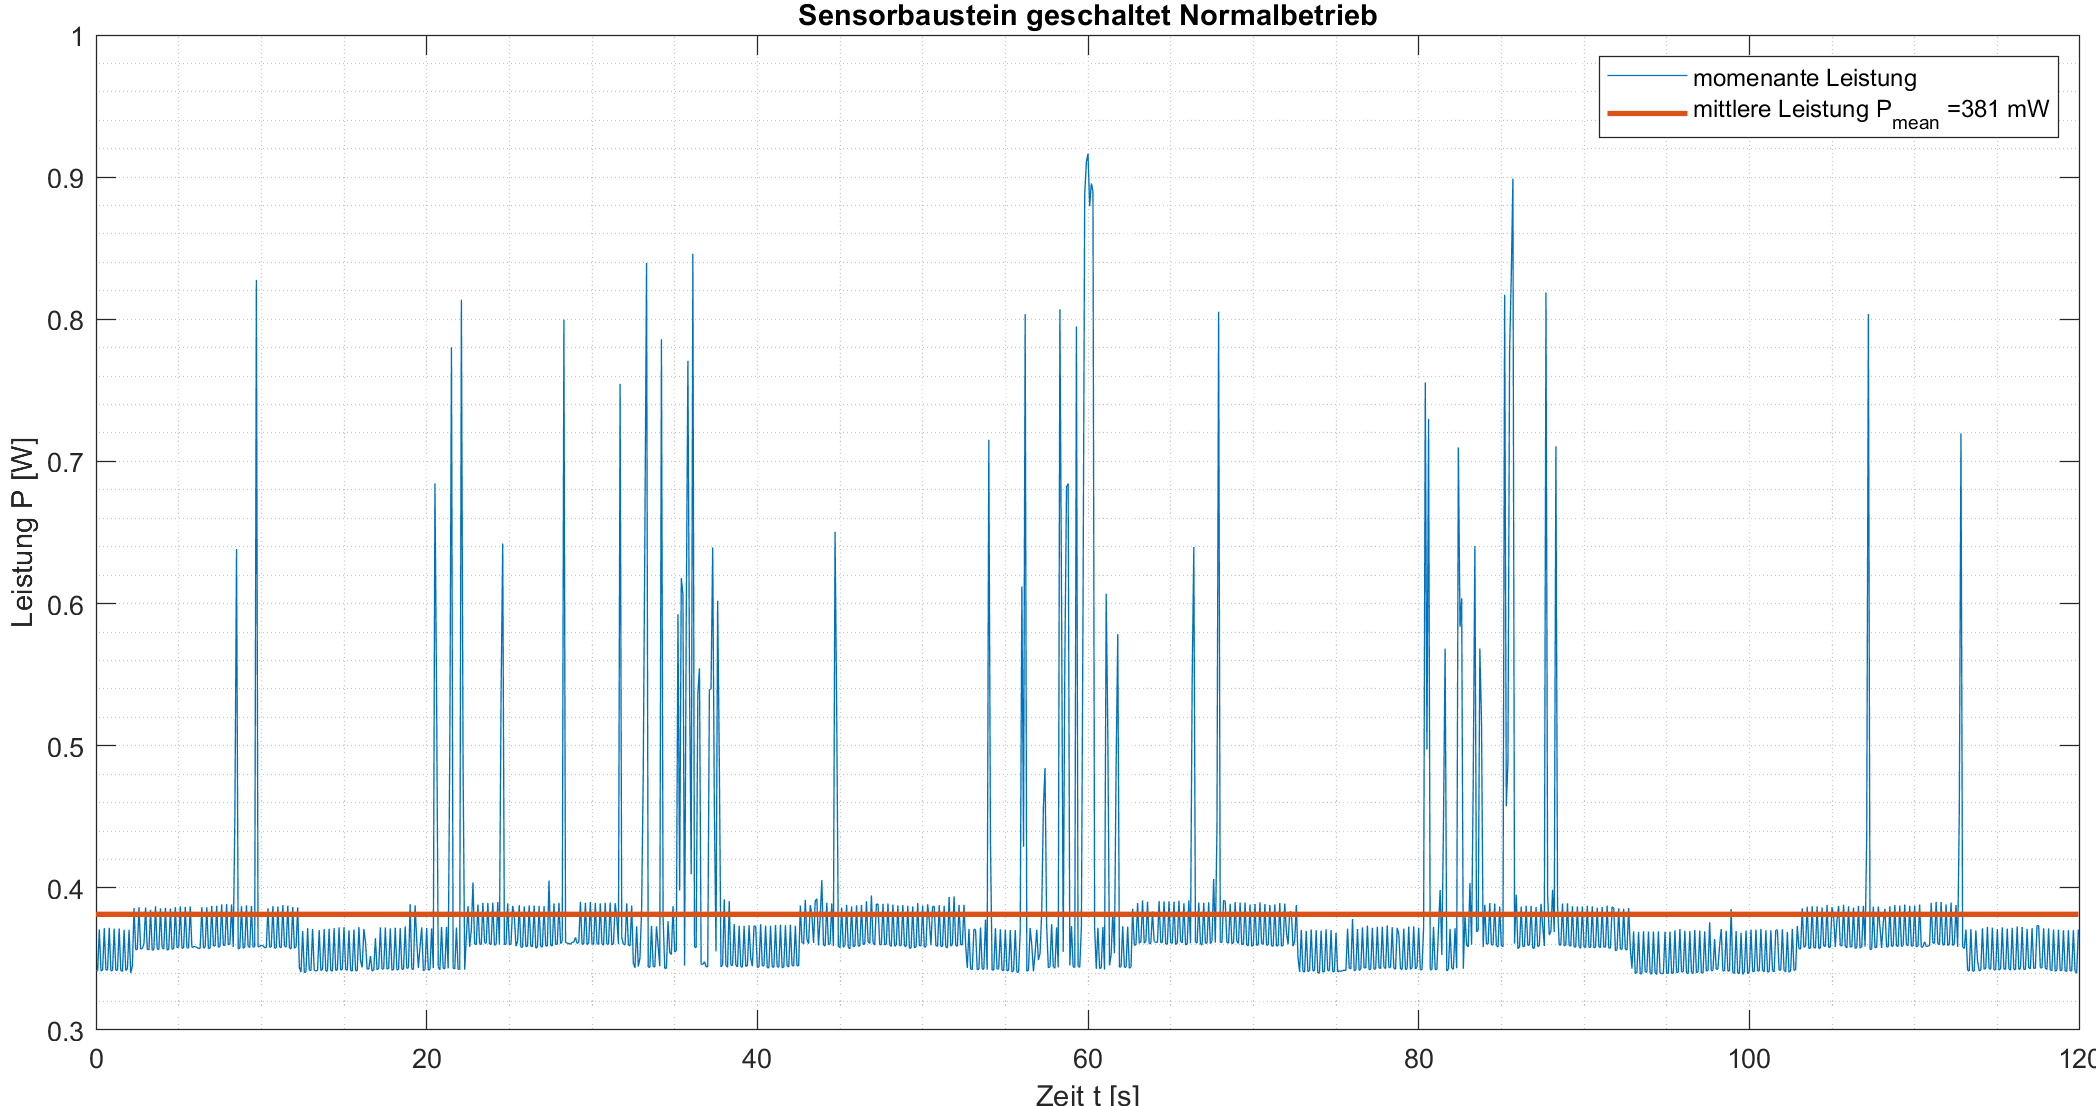
\includegraphics[width=1\textwidth]{graphics/Sensorbaustein_geschaltet.png}
	\caption{Die Leistung des Sensorbausteins, wenn er bedient wird und mit dem Netzwerk verbunden ist}
	\label{pic: Sensorbaustein_geschaltet}
\end{figure}

\begin{figure}[H]
	\centering
	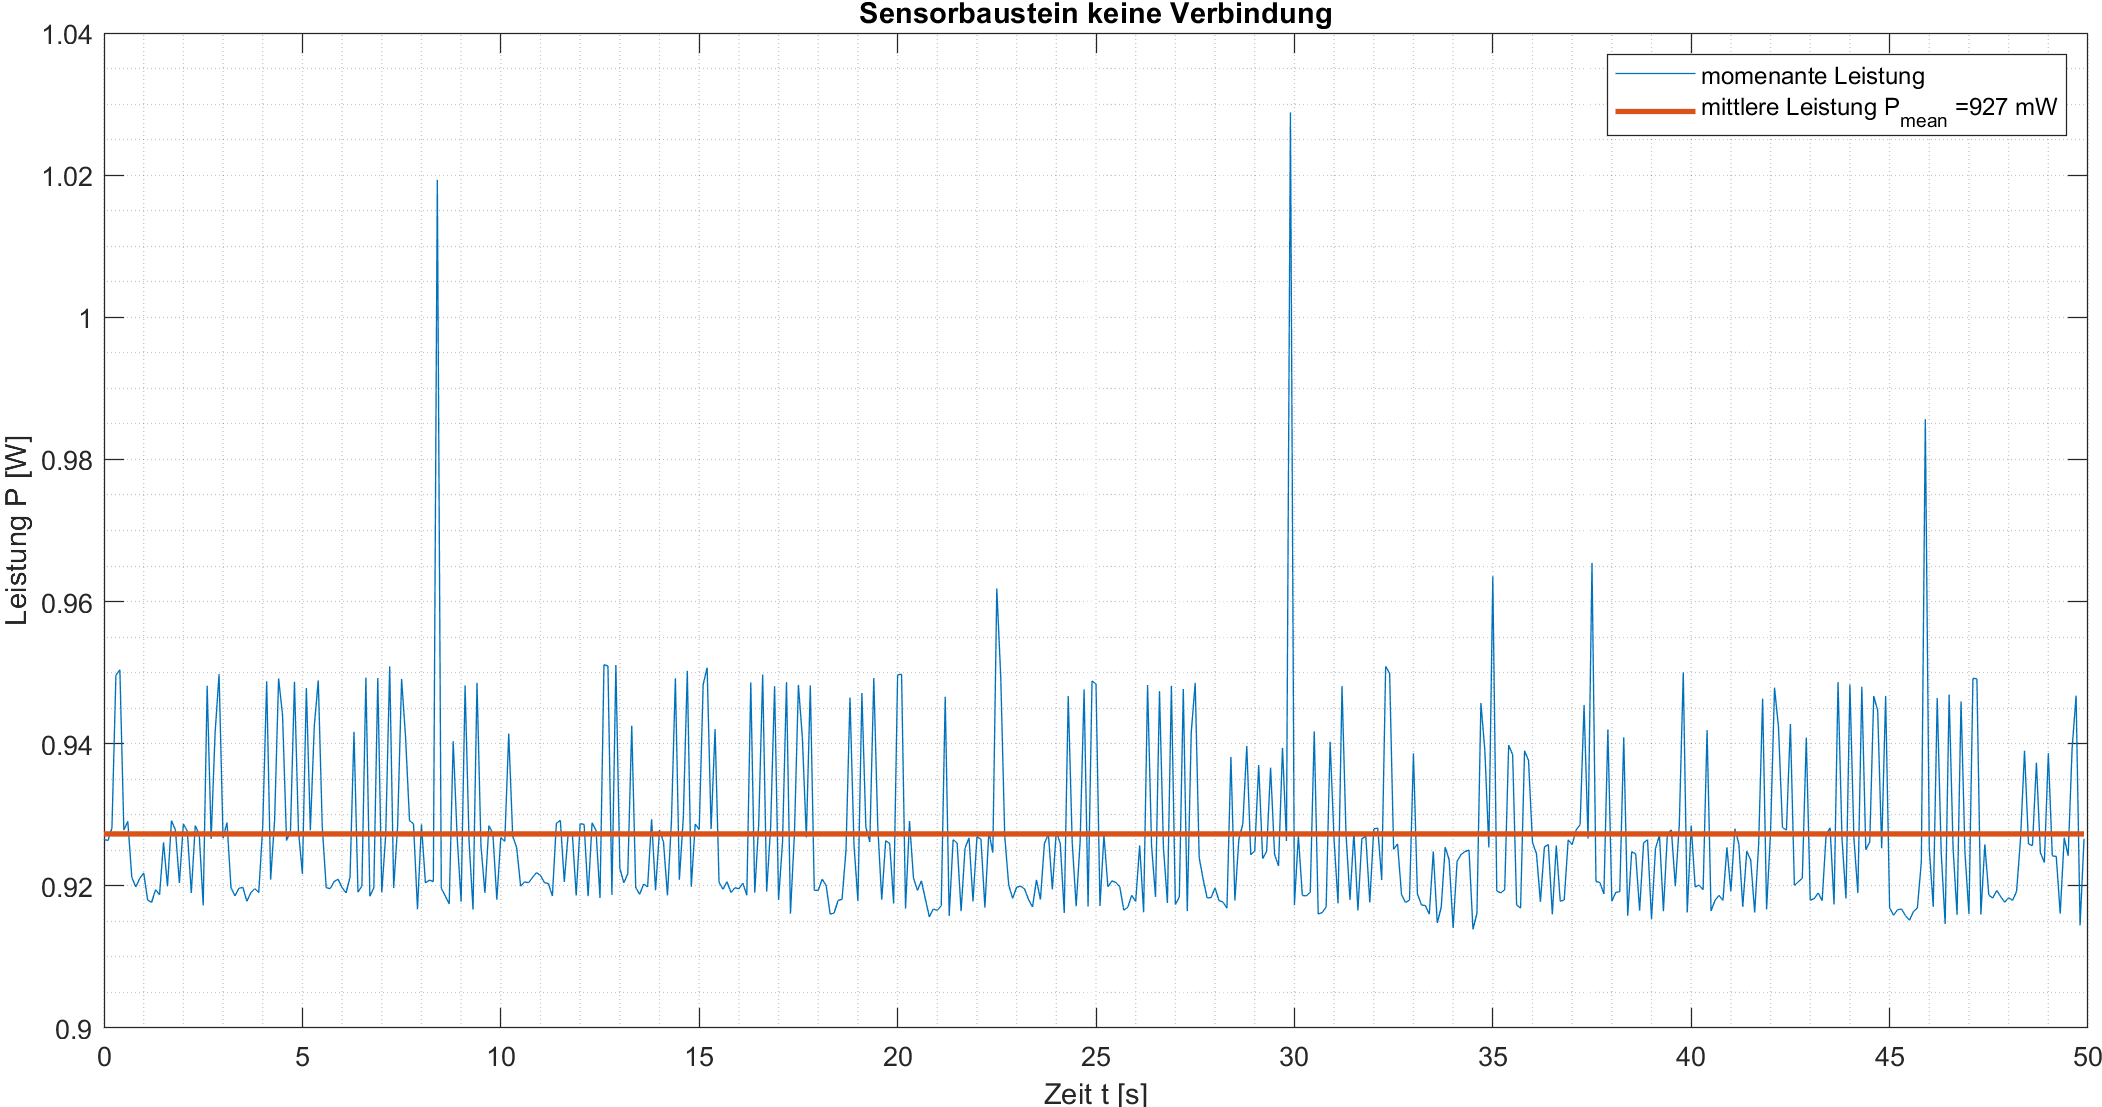
\includegraphics[width=1\textwidth]{graphics/Sensorbaustein_keine_Verbindung.png}
	\caption{Die Leistung des Sensorbausteins, wenn er einen Verbindungsaufbau versucht, aber kein geeignetes WLAN Netzwerk vorhanden ist}
	\label{pic: Sensorbaustein_keine_Verbindung}
\end{figure}




\subsubsection{Temperaturmessung} \label{Temperaturmessung}
Es wird berechnet, wie gross ungefähr die Abweichung der Temperaturmessung um die Raumtemperatur von Wohngebäuden, was üblicherweise 20\,°C entspricht, ist. Dazu wurde mit $U_\text{ref} = 2.39\,V$ und einer Temperatur von 20.2\,°C $\approx$ 20\,°C  gerechnet (folglich Kapitel \ref{tempf}). Gerechnet wird mit einem Vorwiderstand $R_{\text{V}}$ von $100\,k\Omega$ mit 0.1\,\% Abweichung und einem NTC (NCU18WF104J60RB von Murata) mit einem Widerstand von $R_{\text{T}}$, bei welchem der Widerstand R$_{25}$ bei 25\,°C eine Abweichung von 5\,\% hat. Um die Abweichung zu berechnen, wird die anliegende Spannung bei 20.2\,°C berechnet (Gl.: \ref{eq: U_{ntc,20.2,max}}). Um $U_{ntc,max}$ zu maximieren, wurde der maximale Widerstand des NTC bei 20.2\,°C und der kleinst anliegende Wert von dem Vorwiderstand $R_V$ verwendet. Danach wurden mit \ref{eq: R_T/R_V_{max}} und \ref{eq: T_{min}} die Temperatur berechnet. Die Abweichung ergab sich aus der Differenz, des zu erwartenden und des zu berechnenden Wertes, was 0.9\,K entspricht. Da dieser Wert zu hoch erscheint, grösser als 0.5\,°C, wäre ein NTC mit geringerer Toleranz besser gewesen. Dazu gibt es Baugleiche NTCs mit den gleichen Parametern, einfach kleinere Toleranzen.
\\
Werte:
\begin{align*}
R_{T,20.2} &= 126\,k\Omega\\
R_{T,20.2,max} &= 126\,k\Omega \cdot 1.05 = 132\,k\Omega\\
R_V &= 100\,k\Omega\\
R_{V,min} &= 100\,\Omega \cdot 0.99 = 99.9k\,\Omega\\
B &= 4250\,K\\
T_{25} &= 298.15\,K\\
\end{align*}
\\
Was als erhöhte Spannung an $U_{ntc}$ bei 20.2\,°C anliegt:
\begin{align}
U_{ntc,max} &= U_{\text{ref}} \cdot \frac{R_{T,20.2,max}}{R_{T,20.2,max}\;+\;R_{V,min}} = 2.39\;V \cdot \frac{ 132\,k\Omega}{(132\,k\Omega\;+\;99.9\,k\Omega)} = 1.36\,V\label{eq: U_{ntc,20.2,max}}
\end{align}
\\
Temperatur Berechnung bei 20.2\,°C im Mikrocontroller:
\begin{align}
\Biggl( \frac{R_T}{R_V}\Biggr)_{max} &= \frac{U_{ntc,max}}{U_{ref}\;-\;U_{ntc,max}} = 1.32 \label{eq: R_T/R_V_{max}}\\
T &= \frac{1}{\frac{1}{T_{25}}+\frac{1}{B} \cdot ln\Biggl( \Biggl( \frac{R_T}{R_V}\Biggr)_{max}\Biggr)} = 292.45\,K = 19.3\,\,^\circ C \label{eq: T_{min}}\\
\Delta T_{max} &= 20.2\,^\circ C - 19.3\,^\circ C = 0.9\,K \label{dT_{max}}
\end{align}

\subsection{Aktorbaustein} \label{energie_aktorbaustein}
\subsubsection{Energieverbrauch des Aktorbaustein}
Der Aktorbaustein wurde unter folgenden Bedingungen gemessen:

\begin{enumerate}
	\item Ungeschalteter Normalzustand (Abbildung: \ref{pic: Aktorbaustein_ungeschaltet}) \\(Der Aktorbaustein wird nicht bedient und hat eine Verbindung mit einem WLAN Netzwerk) \\
	Der Aktorbaustein hat eine mittlere Leistungsaufnahme von ca. 629\,mW. Auffällig ist, wie beim Sensorbaustein, dass die Leistung mit einer Periode von 10\,s schwankt, was wiederum, wegen des blinkenden Status LED ist. Dazu kommt es alle 10\, zu kurzen Leistungssprüngen.
	\\
	\item Geschalteter Normalzustand (Abbildung: \ref{pic: Aktorbaustein_geschaltet})\\ (Der Aktorrbaustein wird bedient und hat eine Verbindung mit einem WLAN Netzwerk)\\
	Die Relais werden nacheinander eingeschalten und danach wieder ausgeschaltet, ein eingeschaltetes Relais und ein LED verbrauchen zusammen somit ca. (900\,mW - 620m\,W)/4 = 70\,mW.
	\\
	\item Keine Verbindung (Abbildung: \ref{pic: Aktorbaustein_keine_Verbindung})\\ (Der Aktorbaustein findet kein zulässiges WLAN Netzwerk)\\
	In diesem Zustand hat der Aktorbaustein eine mittlere Leistungsaufnahme von 1020\,mW, was ähnlich viel wie beim Sensorbaustein ist, die Ursachen hierfür werden die gleichen sein.
	\\
	\item Keine Verbindung (Abbildung: \ref{pic: Aktorbaustein_Sparmodus})\\ (Der Aktorbaustein schaltet alle Relais einmal mit und einmal ohne Sparmodus)\\
	Zu erwarten ist, dass der Sparmodus ca. 1.5W einspart, denn der eingestellte Dutycycle beträgt 30\,\%, und ein Relais (G5LE-1-VD DC24) verbraucht 400\,mW, wenn es mit 24\,V betrieben wird. Somit ergibt sich aus der Glaichung \ref{eq: P_{gespart,theoretisch}} eine Erparnis von 1.5\,W. In der Grafik ist im Vergleich dazu eine Ersparnis von 1.7\,W (Gl.:  \ref{P_{gespart, gemessen}}). Der Unterschied ist daher, dass der ausgegebene Dutycycle nicht ganz genau 30\,\% und die Amplitude nicht ganz genau 24\,V beträgt.
\end{enumerate}

\begin{align}
P_\text{gespart,theoretisch} &= (1-0.3^2) \cdot 4 \cdot 400\,mW = 1.5\,W \label{eq: P_{gespart,theoretisch}} \\
P_\text{gespart, gemessen} &= 2680\,mW - 940\,mW = 1.7\,W \label{P_{gespart, gemessen}}
\end{align}

\begin{figure}[H]
	\centering
	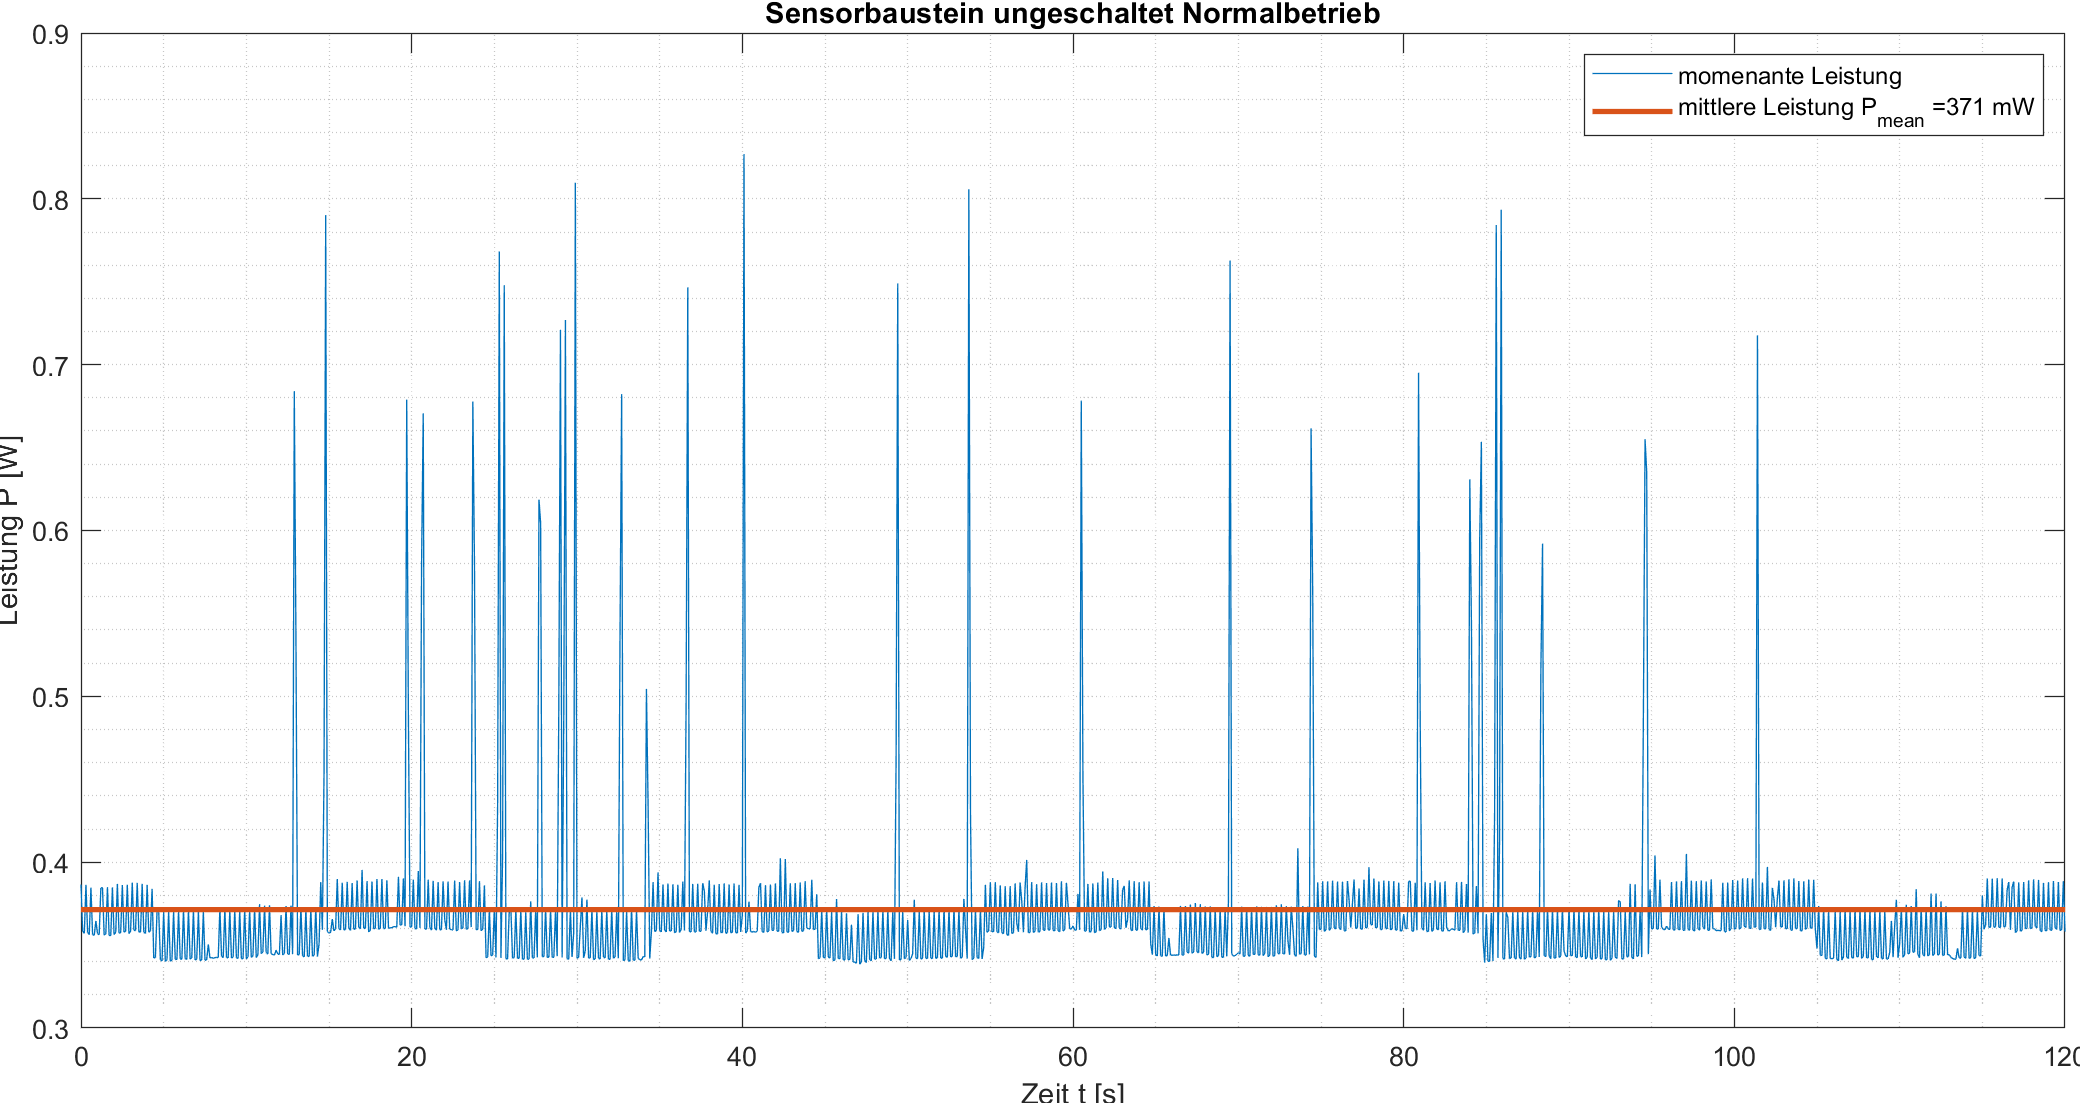
\includegraphics[width=1\textwidth]{graphics/Aktorbaustein_ungeschaltet.png}
	\caption{Die Leistung des Aktorbausteins, wenn er nicht bedient wird und mit dem Netzwerk verbunden ist}
	\label{pic: Aktorbaustein_ungeschaltet}
\end{figure}

\begin{figure}[H]
	\centering
	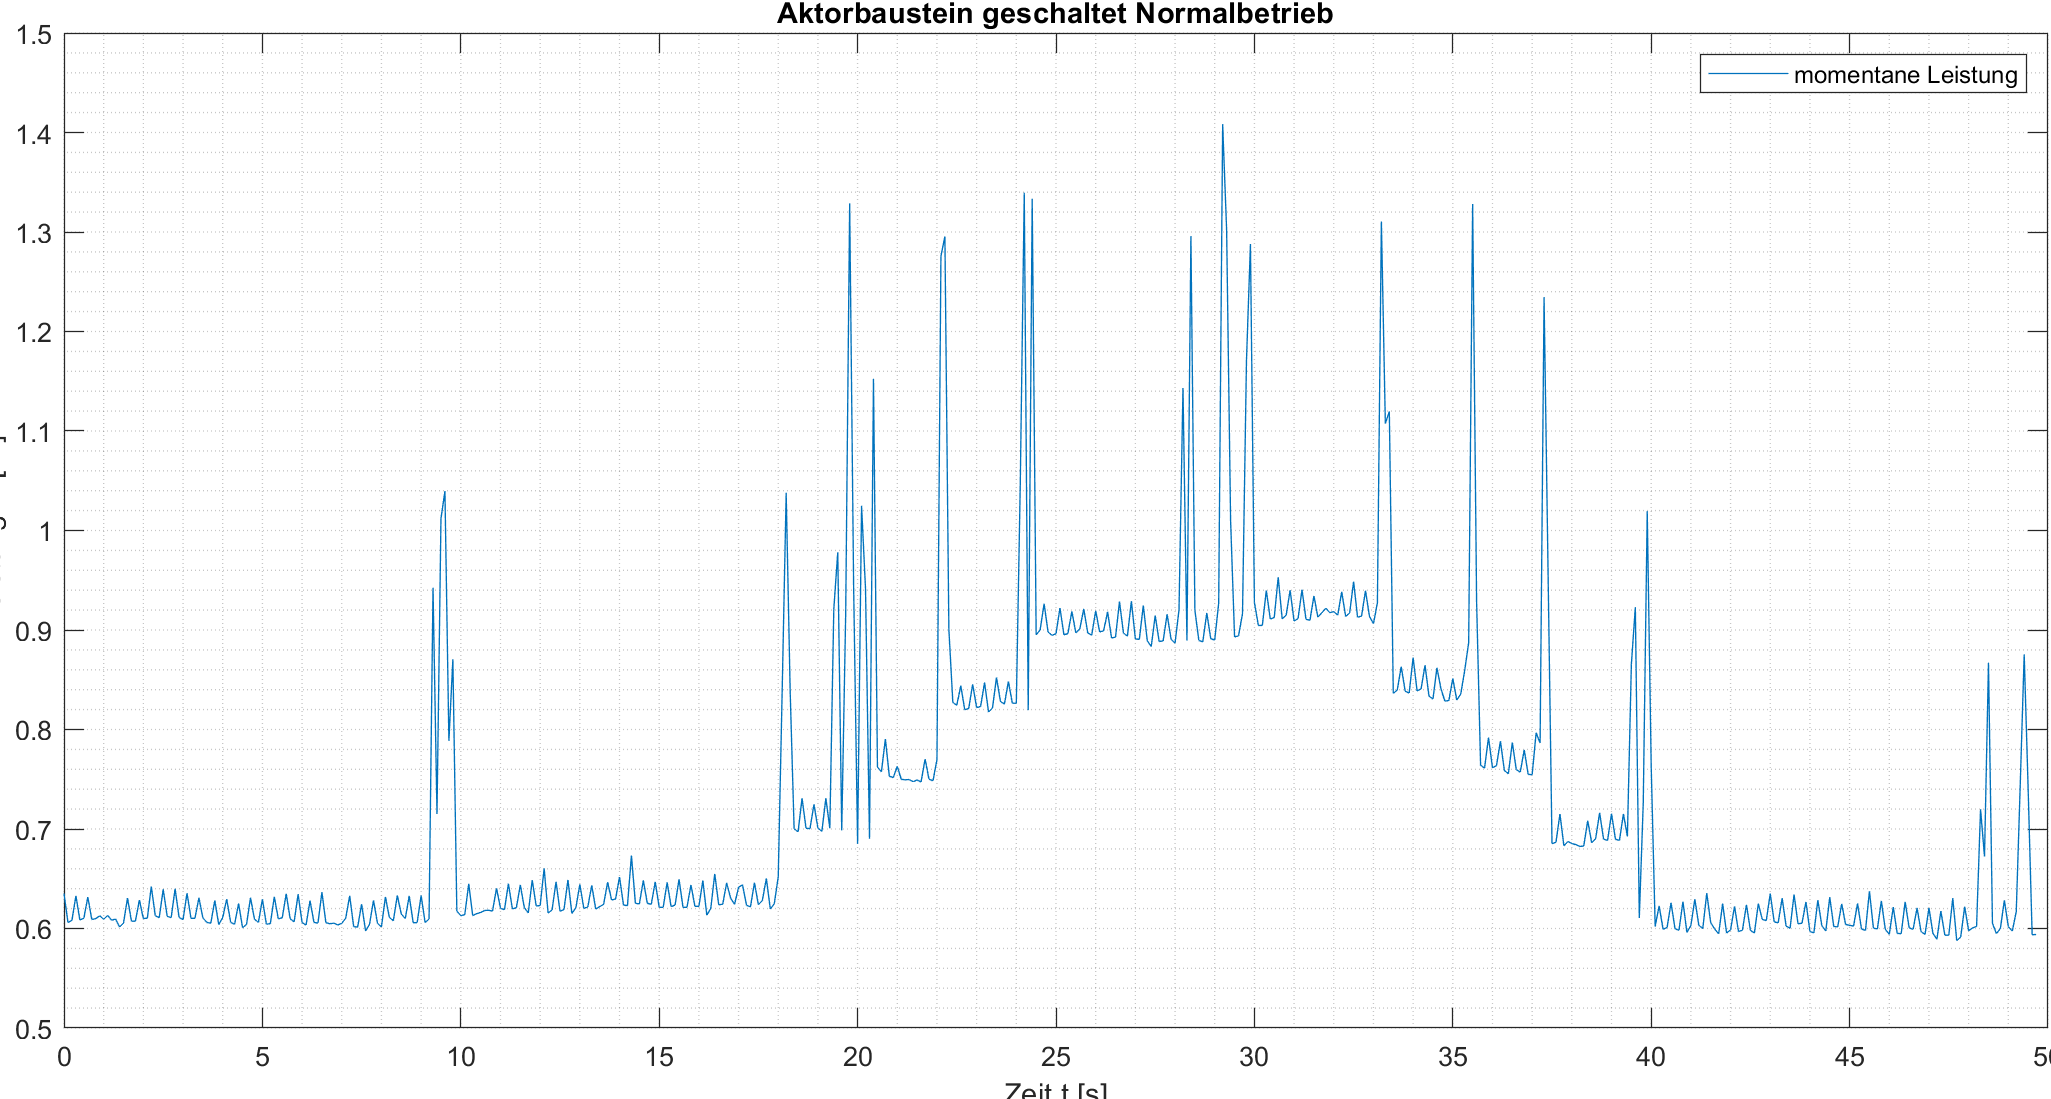
\includegraphics[width=1\textwidth]{graphics/Aktorbaustein_geschaltet.png}
	\caption{Die Leistung des Aktorbausteins, wenn er bedient wird und mit dem Netzwerk verbunden ist}
	\label{pic: Aktorbaustein_geschaltet}
\end{figure}

\begin{figure}[H]
	\centering
	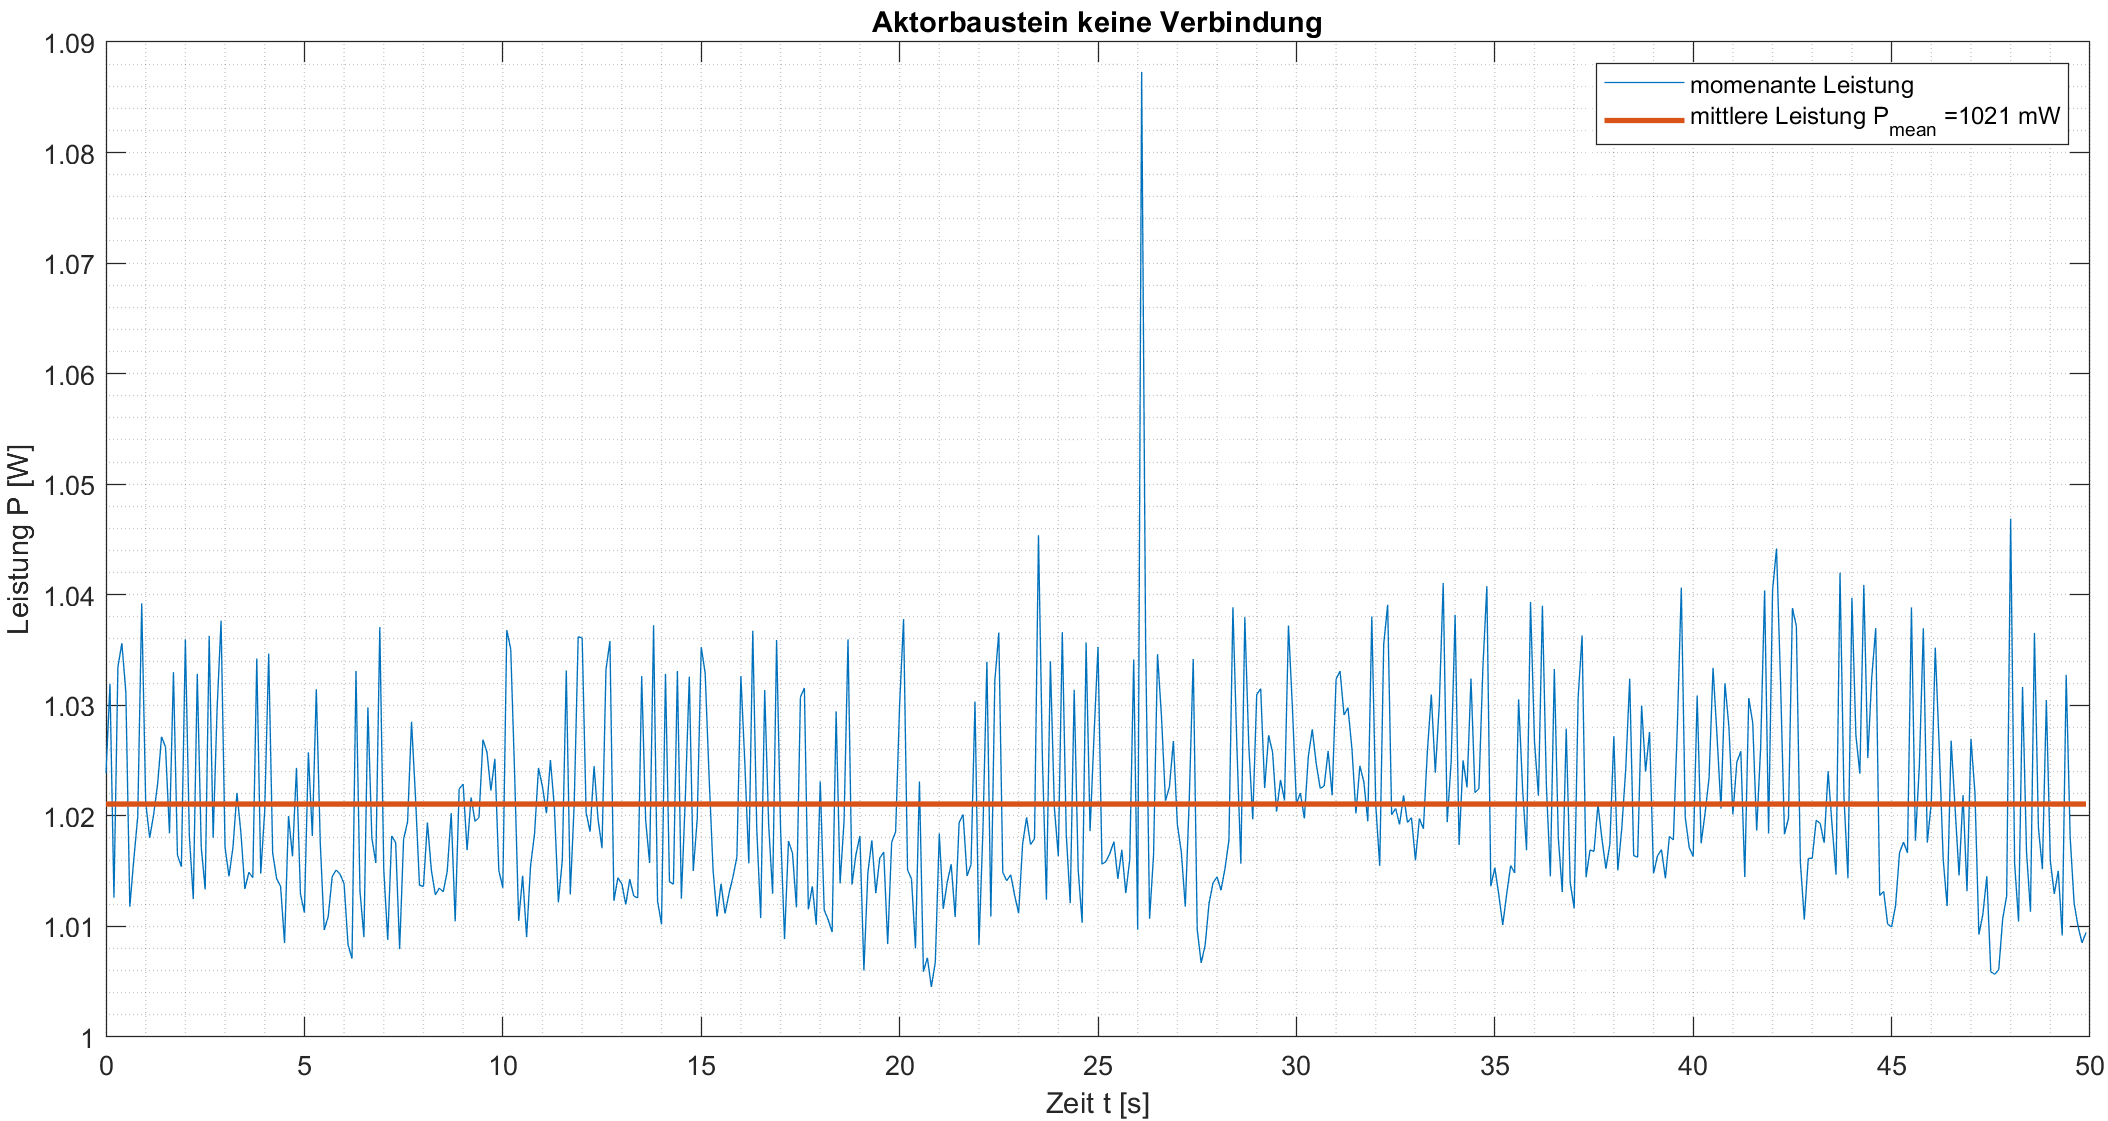
\includegraphics[width=1\textwidth]{graphics/Aktorbaustein_keine_Verbindung.png}
	\caption{Die Leistung des Aktorbausteins, wenn er einen Verbindungsaufbau versucht, aber kein geeignetes WLAN Netzwerk vorhanden ist}
	\label{pic: Aktorbaustein_keine_Verbindung}
\end{figure}

\begin{figure}[H]
	\centering
	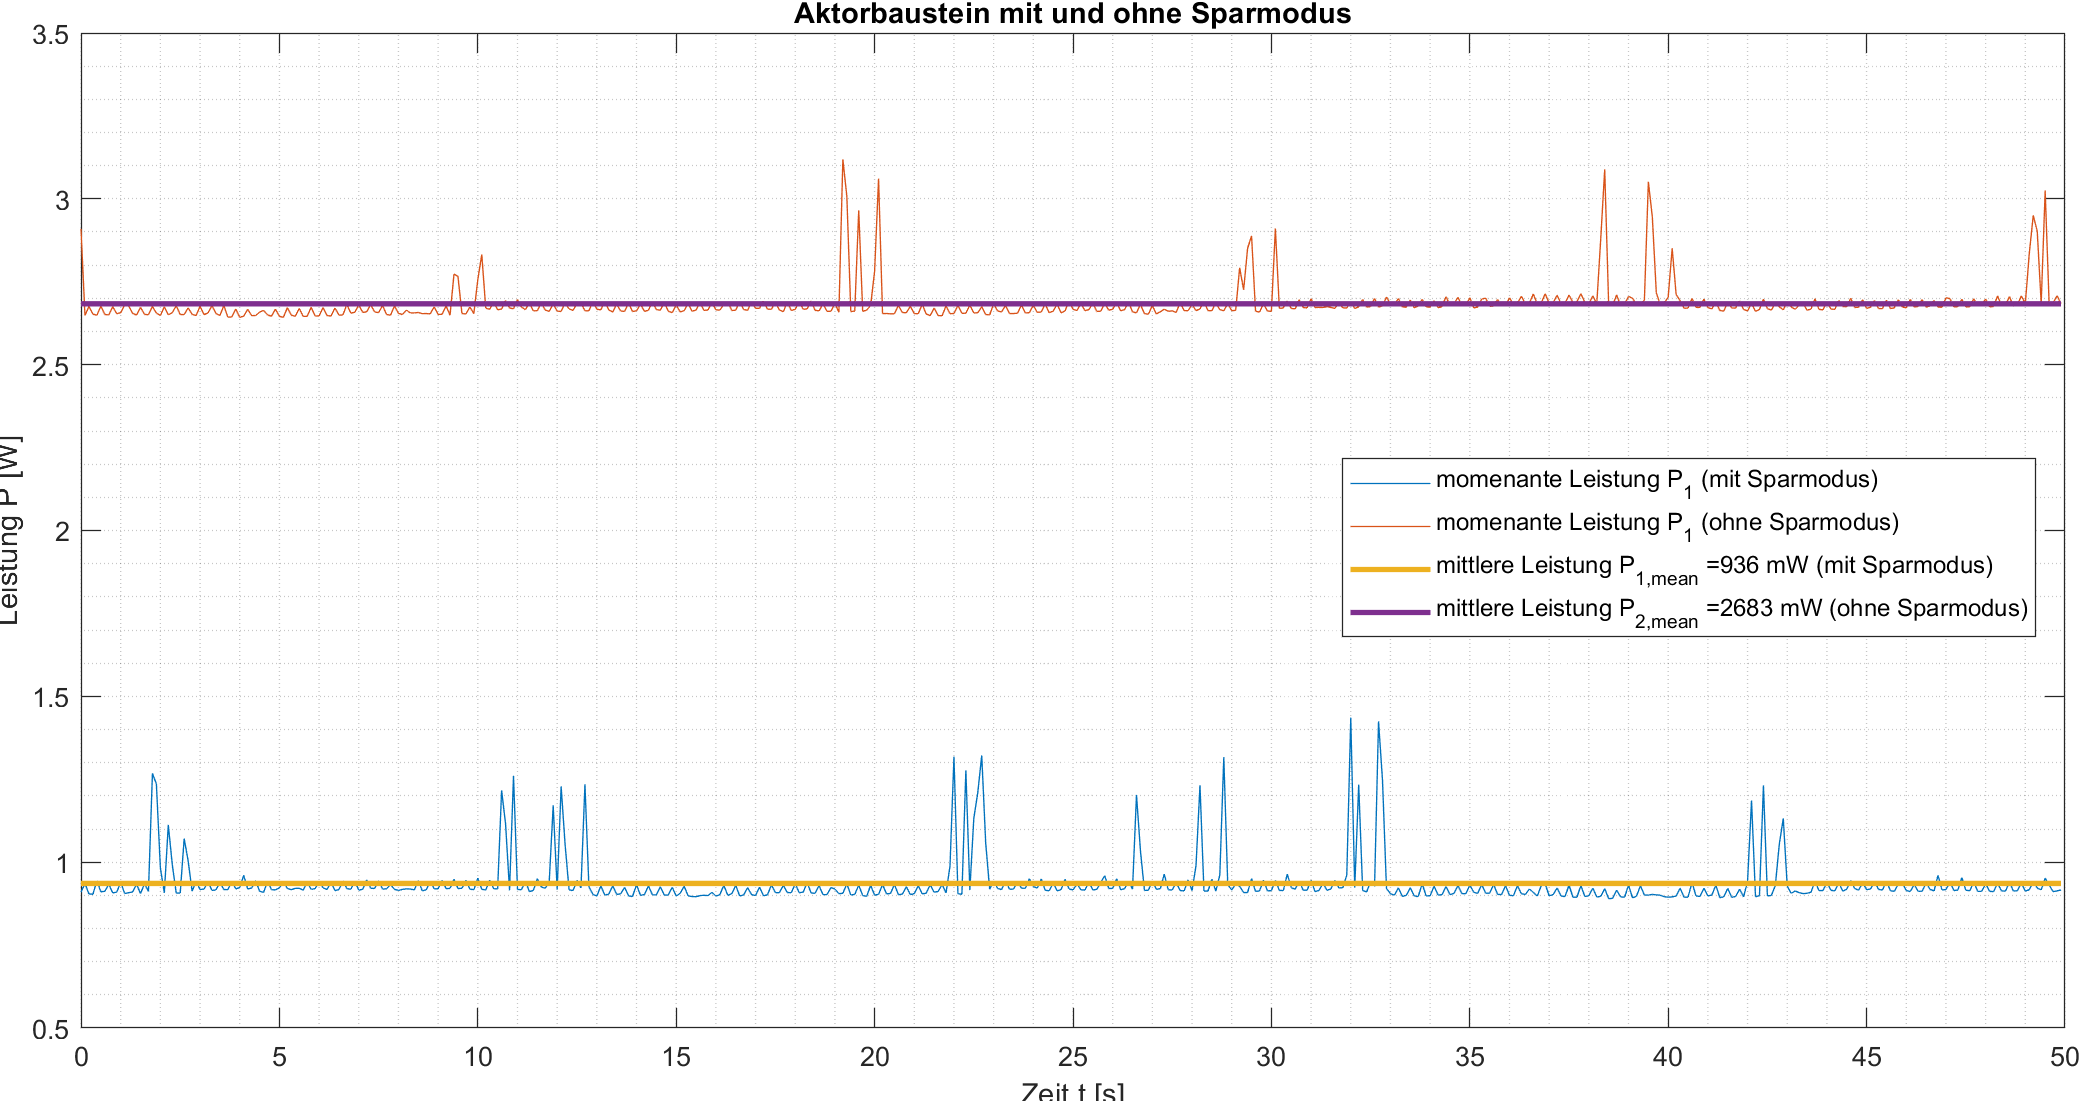
\includegraphics[width=1\textwidth]{graphics/Aktorbaustein_Sparmodus.png}
	\caption{Die Leistung des Aktorrbausteins mit und ohne Sparmodus, wenn er alle Relais schaltet}
	\label{pic: Aktorbaustein_Sparmodus}
\end{figure}

\subsubsection{Wärmeverteilung}
Es wurde verifiziert, wie stark sich der Aktorbaustein in Betrieb erwärmt. Hierfür wurde eine Infrarotkamera von Flir verwendet. Erwärmt haben sich bei normalen Betrieb insbesondere die Diode D14 (Abbildung: \ref{pic: IR_Diode}), der ESP32 (Abbildung: \ref{pic: IR_ESP}) und der DC/DC-Wandler (Abbildung: \ref{pic: IR_Wandler}). Um zu verifizieren wie stark sich die Relaisschaltung erwärmt, wurde eine Last von 9.2\,A 230\,VAC über ein Relais geschaltet, laut Infrarot Kamera wurde eine Temperatur von 58\,°C gemessen, was mit unbestimmten Unsicherheiten zu verstehen ist.


\begin{figure}[htb]
	\centering
	\begin{minipage}[t]{0.45\linewidth}
		\centering
		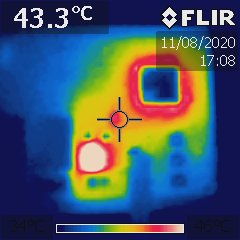
\includegraphics[width=0.9\textwidth]{graphics/IR_Diode.jpg}
		\caption{Wärmeentwicklung über der Diode D14}
		\label{pic: IR_Diode}
	\end{minipage}% <- sonst wird hier ein Leerzeichen eingefügt
	\hfill
	\begin{minipage}[t]{0.45\linewidth}
		\centering
		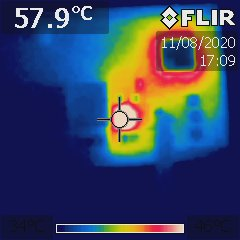
\includegraphics[width=0.9\textwidth]{graphics/IR_Wandler.jpg}
		\caption{Wärmeentwicklung über dem DC/DC-Wandler}
		\label{pic: IR_Wandler}
	\end{minipage}
\end{figure}

\begin{figure}[htb]
	\centering
	\begin{minipage}[t]{0.45\linewidth}
		\centering
		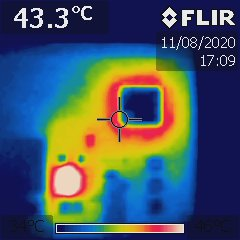
\includegraphics[width=0.9\textwidth]{graphics/IR_ESP.jpg}
		\caption{Wärmeentwicklung über dem ESP32}
		\label{pic: IR_ESP}
	\end{minipage}% <- sonst wird hier ein Leerzeichen eingefügt
	\hfill
	\begin{minipage}[t]{0.45\linewidth}
		\centering
		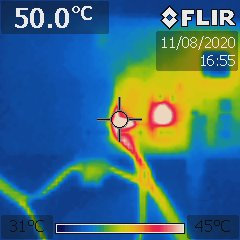
\includegraphics[width=0.9\textwidth]{graphics/IR_Relais.jpg}
		\caption{Wärmeentwicklung über ein Relais welches 9.2\,A / 230\,VAC schaltet}
		\label{pic: IR_Relais}
	\end{minipage}
\end{figure}

\subsubsection{Reaktion Zeiten}
Die Reaktionszeiten von Taster Betätigung auf dem Touch Sensor bis die Schalthandlung am Relais auf dem Aktor Bord  Ausgeführt wird, wurde in nachfolgender Messung ermittelt. 
\begin{figure}[H]
	\centering
	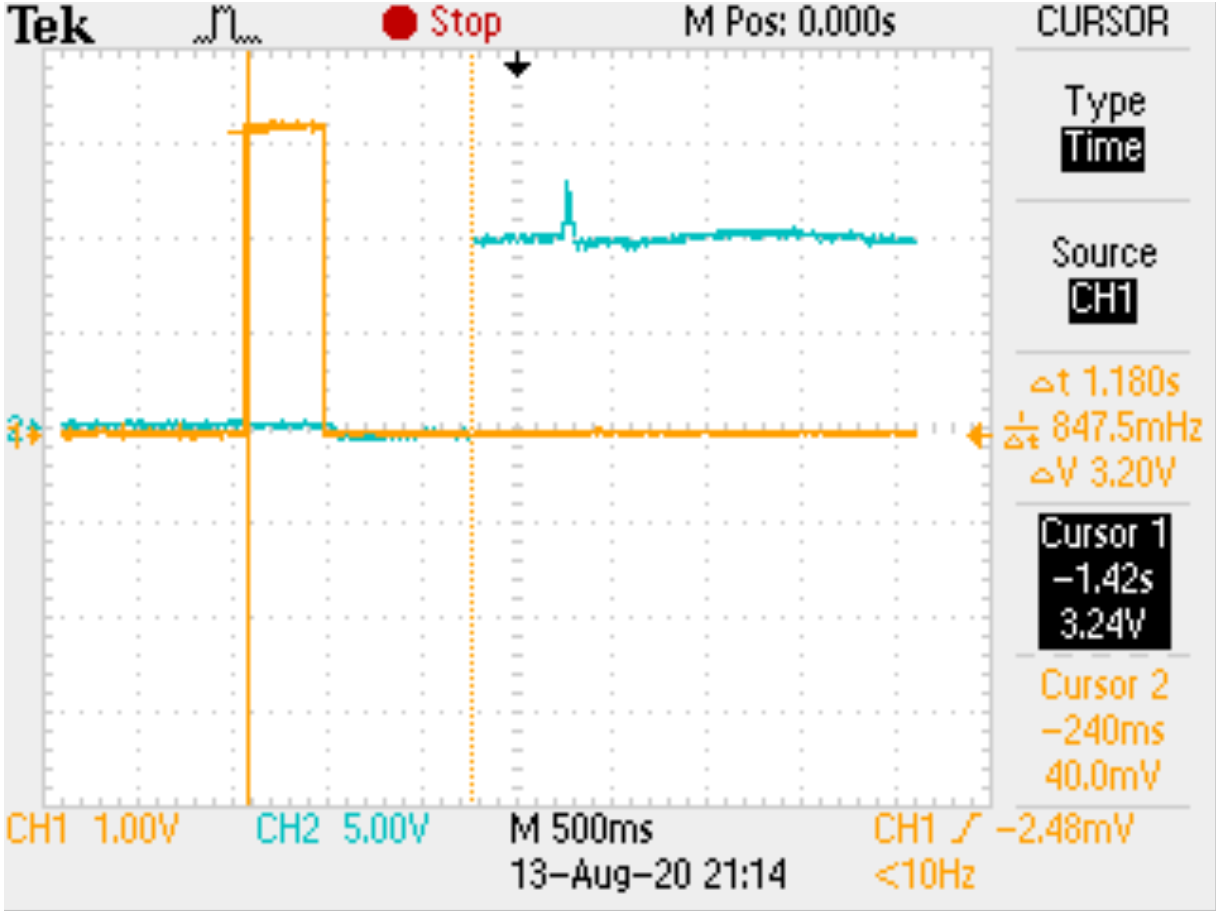
\includegraphics[width=0.75\textwidth]{graphics/ZeitmessungOH.PNG}
	\caption{Signal Taster ist gelb dargestellt, Signal Relais blau dargestellt}
	\label{pic: Zeitmessung Openhab}
\end{figure}
In der Abbildung \ref{pic: Zeitmessung Openhab} kann zwischen dem Auslöse-Signal und dem Schalt-Signal eine Zeitdifferenz von 1.18 Sekunden erkannt werden. Der Grund warum so eine grosse Zeitdifferenz entsteht liegt daran, dass Openhab in den Ruls der Schaltbefehl für den Aktor generiert werden muss.\\
\\
\begin{figure}[H]
	\centering
	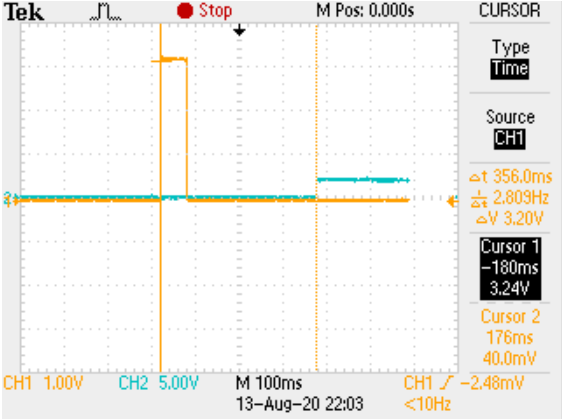
\includegraphics[width=0.75\textwidth]{graphics/ZeitmessungohneOH.PNG}
	\caption{Zeitmessung ohne Openhab Rules, Signal Taster ist gelb und Signal Relais blau dargestellt}
\label{pic: Zeitmessung ohne Openhab}
\end{figure}
In der Abbildung \ref{pic: Zeitmessung ohne Openhab} kann zwischen dem Auslöse-Signal und dem Schalt-Signal eine Zeitdifferenz von 356 ms erkannt werden. Bei dieser Messung wurde der Schaltbefehl, also Topic und Payload im Sensor-Programmcode so angepasst, dass direkt eine Schalthandlung ausgelöst wird, sprich Rules von Openhab wurden umgangen.

\subsubsection{Absicherungen}
Es werden verschiedene Sicherheitselemente des Aktorbausteins überprüft.

\paragraph{Kurzschluss an den Ein- und Ausgängen}\\
Falls die 10\,V Ausgänge kurzgeschlossen werden, nimmt der Aktorbaustein keinerlei schaden, da der Kurzschlussstrom begrenzt wird durch die Widerstände R15 und R16. Es wurde bei 10\,V als Output definiert und das Signal auf mit Ground verbunden, das Ergebnis war ein Kurzschlussstrom von 21.7\,mA. (Abbildung: \ref{pic: Output_aktor}).

\paragraph{Verpolungsschutz Speisung}\\
Falls die Klemmen für die Speisung verwendet werden, wird der Strom über die Diode D15 auf die PPTC Sicherung gelangen. Dies wurde getestet und die Sicherung wurde heiss und begrenzte so den Strom, der Aktorbaustein hat unbeschadet überstanden.


\paragraph{Kurzschluss an den Ein- und Ausgängen}\\


